
\documentclass[paper-main.tex]{subfiles}
\begin{document}


\begin{figure*}
	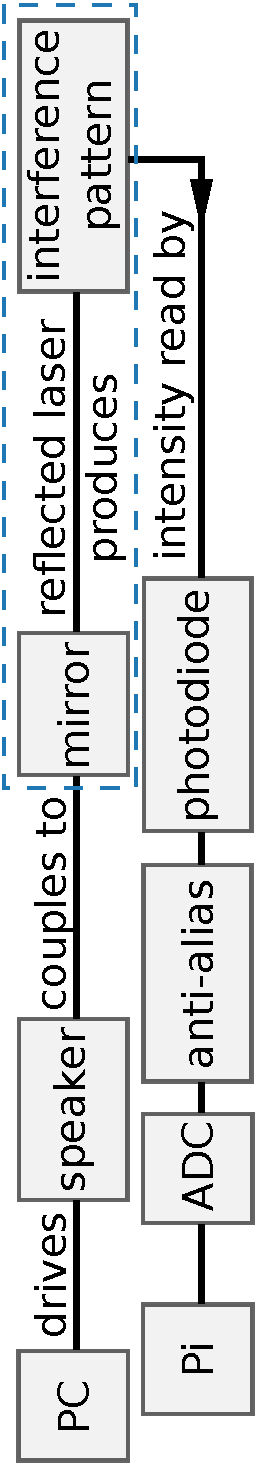
\includegraphics[height=.8\textwidth, angle=-90]{figures/pipeline.pdf}
	\caption{\label{fig:pipeline_highlighted}
Flowchart for the signal through the optical microphone. The transfer function would have to account for each stage. 
The stage inside the blue-dashed box is analyzed in Appendix~\ref{app:intensity_derivation}. Understanding the other stages is one aim of future work. Not shown are the signal processing filters that are performed on the PC once the data is transferred off the Pi.
}
\end{figure*}

The optical microphone experiment described here can be used to demonstrate and teach a variety of topics, including basic optics and photodiode circuits, to signals processing and speech enhancement. Here, we consider further extensions and improvements to the experiment such as noise isolation, transfer function analysis, speech recognition, and control systems.



Isolating the experiment from interference may provide some noise reduction. 
For example, the Raspberry Pi could be powered with a commercial battery instead of mains power. 
All other components of the circuit draw power from the Pi, so this would isolate the circuit from the mains. 
The laser is DC-powered through a converter, so the laser should not couple noise from the mains into the interferometer. 
Transferring the circuit from a breadboard to a printed circuit board can also reduce interference~\cite{elfekey2013design}.
A feedback loop control system can also be used to suppress any unwanted movement of the interferometer components~\citep{abbott2017exploring, Sekiguchi:2016bmv, verhoeven2009robust}, similar to methods used to isolate gravitational-wave observatories. 





A thorough characterization of the system's transfer function would allow us to understand how audio signals couple through the interferometer. 
The total transfer function starts with the voltage being sent to the speaker and ends with the voltage recorded by the Pi. It also would include any inherent non-linearities in the speaker, the speaker-mirror coupling, the path length to intensity relation (Appendix~\ref{app:intensity_derivation}), and the photodiode. The schematic in Fig.~\ref{fig:pipeline_highlighted} shows the abstract signal flow through the system.
It does not include other potential pathways for signal flow such as acoustomechanical vibrations of the webcam or photodiode mount which could also be examined.
% commented out whilst James is checking this
% jam: I'm pretty confident this is what Rob said. 
%With perfect knowledge of the transfer function, signal recovery is limited by the signal-to-noise ratio as an optimal matched filter could be constructed.
%\jam{[check with Rob et al. about the veracity of this]}

A voluminous literature exists on using hidden Markov models trained on phonemes to recognize speech~\cite{HMM_english}. These could perform the final stage of speech enhancement for the optical microphone. Interestingly, this coincidentally connects back to the Viterbi algorithm in Section~\ref{sec:viterbi_wandering}, which is also underpinned by a hidden Markov model, albeit of a different type. Alternatively, machine learning solutions exist throughout the field that can compete with statistical techniques such as the logMMSE estimator~\cite{SEGAN}.


We could also use more traditional techniques such as a wavelet transform (WT) \citep{nason1995stationary} to extract the signal from noise, and compare these with the above methods. A WT provides both time and frequency information, making it easier to pinpoint the origin of noise with respect to time. In Refs.~\cite{tufekci2000feature,agbinya1996discrete}, WT methods are proposed for speech recognition. 

Returning to the demonstration of continuous gravitational-wave analysis, further extensions could include analyzing data from multiple interferometers to extract directional information for audio signals. 
This would require increasing the sensitivity of the optical microphone to pick up the signal from a distant source instead of from a speaker attached directly to one of the mirrors of the interferometer.
Another extension would be to demonstrate the Doppler effect of the Earth's motion around the Sun, which needs to be considered in continuous-wave searches (see Section~\ref{sec:realCWSearches} and Ref.~\cite{JKS:1998}). 
One approach could be to move either the interferometer or the source signal on a circular track or modify the input audio signal to simulate Doppler modulation. 
%techniques used in the literature to address it by moving the optical table on some kind of circular track with period far shorter than the time it takes the signal to significantly wander in frequency. Then, by placing a distant signal source at different positions above or beside the track -- or perhaps more practically the source could move instead of the detector, an analogous Doppler effect could be observed.



\end{document}
